\section*{Exercise 8a}

{
\bfseries 
Let $I$ be the input image in file \texttt{isn\_256.pgm}, which has a binary impulsive noise added(``salt-and-pepper'' noise). Let $B$ be a structuring element square of size $3 \times 3$.
}

The results of executing the respective filters can be seen in Fig. \ref{fig:exercise_8a_images}. The best results are obtained using Filter \hyperref[fig:exercise_8a_ope_clo]{4} (Opening-Closing $\gamma\varphi$) where it is easy to see there is only one artifact left in the image (on top of the black part).

The second best filter is Filter \hyperref[fig:exercise_8a_clo_ope]{3} (Closing-Opening $\varphi\gamma$) where a few more artifacts remain in the image, in this case, in the white part.

As we can see in Filters \hyperref[fig:exercise_8a_ope]{1} (Opening $\gamma$) and \hyperref[fig:exercise_8a_clo]{2} (Closing $\varphi$), each operation removes artifacts from one of the parts, and thus, the combinations of both are the ones that obtain better results.

\begin{figure}[b!]
    \centering
    {
    \captionsetup[subfloat]{labelformat=empty}
    \subfloat[Orignal image: \texttt{isn\_256.pgm}]{\frame{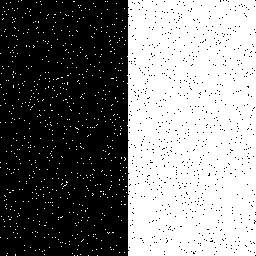
\includegraphics[width=0.4\textwidth]{img/exercise_8a_original.png}}\label{fig:exercise_8a_original}} \\
    }
    \captionsetup[subfloat]{labelformat=simple}
    \renewcommand{\thesubfigure}{Filter \arabic{subfigure}:}
    \addtocounter{subfigure}{-1}
    \subfloat[Opening $\gamma_B(I)$]{\frame{
\includegraphics[width=0.4\textwidth]{img/exercise_8a_ope1.png}}\label{fig:exercise_8a_ope}} \quad
    \subfloat[Closing $\varphi_B(I)$]{\frame{
\includegraphics[width=0.4\textwidth]{img/exercise_8a_clo1.png}}\label{fig:exercise_8a_clo}}
    
    
\end{figure}

\clearpage

\phantom{a}

\begin{figure}[t!]
    \centering
    \captionsetup[subfloat]{labelformat=simple}
    \addtocounter{subfigure}{2}
    \renewcommand{\thesubfigure}{Filter \arabic{subfigure}:}
    \subfloat[Closing-Opening $\varphi_B\gamma_B(I)$]{\frame{
\includegraphics[width=0.4\textwidth]{img/exercise_8a_clo1_ope1.png}}\label{fig:exercise_8a_clo_ope}} \quad
    \subfloat[Opening-Closing $\gamma_B\varphi_B(I)$]{\frame{
\includegraphics[width=0.4\textwidth]{img/exercise_8a_ope1_clo1.png}}\label{fig:exercise_8a_ope_clo}}
    \caption{Images from Exercise 8a}
    \label{fig:exercise_8a_images}
\end{figure}
